\documentclass[12pt,letterpaper]{article}



%%
%% Required packages:
%%
\usepackage{etex}
\usepackage{amsmath}
\usepackage{amssymb}
\usepackage{amstext}
\usepackage{amsthm}
\usepackage{fancyhdr,fancybox}
\usepackage{mathrsfs} % need for \mathscr command
\usepackage{multicol}
\usepackage[normalem]{ulem}
%\usepackage{pictex,pictexplus}
% \usepackage{pictexwd}
\usepackage{rotating}
\usepackage{url}
\usepackage{xfrac}
\usepackage{booktabs}
\usepackage{color,soul}
\usepackage{comment}

\usepackage{hyperref}
\hypersetup{
    colorlinks=true,     % false: boxed links; true: colored links
    linkcolor=blue,      % color of internal links
    citecolor=blue,      % color of links to bibliography
    filecolor=blue,      % color of file links
    urlcolor=blue        % color of external links
}


\usepackage{tikz}
\usetikzlibrary{backgrounds,calc}

%%
%% Common formatting commands
%%
\setlength{\parindent}{0in}
\setlength{\textwidth}{7in}
\setlength{\evensidemargin}{-0.25in}
\setlength{\oddsidemargin}{-0.25in}
\setlength{\parskip}{.5\baselineskip}
\setlength{\topmargin}{-0.5in}
\setlength{\textheight}{9in}

%               Problem and Part
\newcounter{problemnumber}
\newcounter{partnumber}
\newcounter{subpartnumber}
\newcommand{\Problem}{%
  \refstepcounter{problemnumber}%
  \setcounter{partnumber}{0}%
  \setcounter{subpartnumber}{0}%
  \item[\makebox{\hfil\textbf{\theproblemnumber.}\hfil}]%
  }
\newcommand{\InProblem}[2][1.6]{%
  \refstepcounter{problemnumber}%
  \setcounter{partnumber}{0}%
  \setcounter{subpartnumber}{0}%
  \textbf{\theproblemnumber.}\ \ \parbox[t]{#1in}{#2}%
}
\newcommand{\InSmallProblem}[1]{\InProblem[1.05]{#1}}
\newcommand{\NoProblem}[1]{%
  \mbox{\hfil\textbf{#1}\hfil}%
  }
\newcommand{\UnProblem}{%
  \refstepcounter{problemnumber}%
  \setcounter{partnumber}{0}%
  \setcounter{subpartnumber}{0}%
  \mbox{\hfil\textbf{\theproblemnumber.}\hfil}%
  }
\newcommand{\InFlexProblem}[1]{%
  \refstepcounter{problemnumber}%
  \setcounter{partnumber}{0}%
  \setcounter{subpartnumber}{0}%
  \textbf{\theproblemnumber.}\ \ #1%
}
%%  Part:
\newcommand{\Part}{%
  \renewcommand{\thepartnumber}{(\alph{partnumber})}%
  \refstepcounter{partnumber}
  \setcounter{subpartnumber}{0}%
  \item[(\alph{partnumber})]%
}
\newcommand{\InPart}[2][1.75]{%
  \renewcommand{\thepartnumber}{(\alph{partnumber})}%
  \refstepcounter{partnumber}%
  \setcounter{subpartnumber}{0}%
  (\alph{partnumber})\ \ \parbox[t]{#1in}{#2}%
}
\newcommand{\UnPart}{%
  \refstepcounter{partnumber}%
  \renewcommand{\thepartnumber}{(\alph{partnumber})}%
  \setcounter{subpartnumber}{0}%
  (\alph{partnumber})%
}
\newcommand{\InLargePart}[1]{\InPart[3.05]{#1}}
\newcommand{\InFullPart}[1]{\InPart[6.2]{#1}}
\newcommand{\InSmallPart}[1]{\InPart[1.05]{#1}}
%% SubPart:
\newcommand{\SubPart}{%
  \refstepcounter{subpartnumber}%
  \item[(\roman{subpartnumber})]%
  }
\newcommand{\InSubPart}[2][2.25]{%
  \stepcounter{subpartnumber}%
  (\roman{subpartnumber})\ \ \parbox[t]{#1in}{#2}%
}
\newcommand{\InSmallSubPart}[1]{\InSubPart[1.5]{#1}}
\newcommand{\InTinySubPart}[1]{%
  \stepcounter{subpartnumber}%
  (\roman{subpartnumber})\ \ \makebox{#1}%
}
\newcommand{\InMySubPart}[2][2.25]{%
  \stepcounter{subpartnumber}%
  \parbox[t]{#1in}{\makebox[0.3in][l]{(\roman{subpartnumber})}\ \ {#2}}%
}
\newcommand{\TrueFalse}{\textbf{T}\ \ \textbf{F}\ \ }
\newcommand{\TFPart}[1]{% 
  \stepcounter{partnumber}%
  \setcounter{subpartnumber}{0}%
  \item[(\alph{partnumber})] \TrueFalse\parbox[t]{5.5in}{#1}}

\newcommand{\Points}[1]{(#1 points) \ }
\newcommand{\Point}[1]{(#1 point) \ }


%% For Answers:
\newcounter{answernumber}
\newcommand{\Answer}{%
  \refstepcounter{answernumber}%
  \setcounter{partnumber}{0}%
  \setcounter{subpartnumber}{0}%
  \item[\makebox{\hfil\textbf{\theanswernumber.}\hfil}]%
  }


% Setting up the headers for the first page
%\chead{} % will default to what is typed in the file.
\fancyhead[L]{\textsc{Math 22a}}
\fancyhead[R]{\textsc{Fall 2024}}
\fancyfoot[R]{
	\vspace*{\fill}\footnotesize\textcopyright{} \emph{Harvard Math 22a}	
}
\renewcommand{\headrulewidth}{0pt}

%\fancyhead[C]{}
%	\chead{}	
%	\lhead{}
%	\rhead{}
%	\cfoot{}


% Putting copyright on the footer of each page
%\fancypagestyle{secondpage}{
%	\fancyhead[C]{TESTing again} % change this to be blank
%		%\chead{}	
%	\fancyhead[L]{bears} % change this to be blank
%	\fancyhead[R]{dogs} % change this to be blank
%	\fancyfoot[R]{ %keeps the footer the same
%		\vspace*{\fill}\footnotesize\textcopyright{} \emph{Harvard Math 22a}	
%	}
%}
%\renewcommand{\headrulewidth}{0pt}
%\pagestyle{fancy}
\pagestyle{empty}


%\lhead{}
%\rhead{}
%\rfoot{\vspace*{\fill}\footnotesize\textcopyright{} \emph{Harvard Math 22a}}
%\renewcommand{\headrulewidth}{0pt}
%\pagestyle{fancy}




%%
%% Common shortcut commands:
%%
\newcommand{\ds}{\displaystyle}
\newcommand{\sgn}{\operatorname{sgn}}
\renewcommand{\Pr}{\operatorname{P}}
\newcommand{\CPr}[3][{}]{\Pr_{\text{#1}}\left(#2\,|\,#3\right)}

\newcommand{\C}{\mathbb{C}}
\newcommand{\R}{\mathbb{R}}
\newcommand{\Z}{\mathbb{Z}}
\newcommand{\N}{\mathbb{N}}
\newcommand{\Q}{\mathbb{Q}}
\newcommand{\D}{\mathbb{D}}

\newcommand{\rref}{\operatorname{rref}}
\newcommand{\im}{\operatorname{im}}
\newcommand{\rank}{\operatorname{rank}}
\newcommand{\diag}{\operatorname{diag}}
\newcommand{\Span}{\operatorname{span}}
%\renewcommand{\vec}[1]{\mathbf{#1}}
\newcommand{\charpoly}{\mathscr{P}}
\newcommand{\nicefrac}[2]{\sfrac{#1}{#2}} % using xfrac package
\newcommand{\topology}{\mathcal{T}}
\newcommand{\Inn}{\operatorname{Inn}}

\newcommand{\blankbox}[2]{\fbox{\rule{#1}{0in}\rule{0in}{#2}}}

\newenvironment{myindentpar}[1]%
 {\begin{list}{}%
         {\setlength{\leftmargin}{#1}
          \setlength{\rightmargin}{\leftmargin}}%
         \item[]%
 }
 {\end{list}}
\newtheorem{theorem}{Theorem}
\newtheorem*{NStheorem}{Theorem}
\newtheorem{cor}[theorem]{Corollary}
\newtheorem*{claim}{Claim}
\newtheorem{defn}{Definition}

\newenvironment{amatrix}[1]{%
  \left(\begin{array}{@{}*{#1}{c}|c@{}}
}{%
  \end{array}\right)
}

%--------grstep
% For denoting a Gauss' reduction step.
% Use as: \grstep{\rho_1+\rho_3} or \grstep[2\rho_5 \\ 3\rho_6]{\rho_1+\rho_3}
\newcommand{\grstep}[2][\relax]{%
   \ensuremath{\mathrel{
       {\mathop{\longrightarrow}\limits^{#2\mathstrut}_{
                                     \begin{subarray}{l} #1 \end{subarray}}}}}}
\newcommand{\swap}{\leftrightarrow}


\usetikzlibrary{arrows}
\usepackage{wrapfig}

\makeatletter
\renewcommand*\env@matrix[1][*\c@MaxMatrixCols c]{%
	\hskip -\arraycolsep
	\let\@ifnextchar\new@ifnextchar
	\array{#1}}
\makeatother

\def\env@matrix{\hskip -\arraycolsep
	\let\@ifnextchar\new@ifnextchar
	\array{*\c@MaxMatrixCols c}}

\chead{\Large\textbf{A Sequence of Family Weekend Puzzles:}}% 

\begin{document}
\thispagestyle{fancy}

\begin{enumerate}
\item The Math 22 team has an idea to raise funds for next year. We are going to buy 8-inch by 8-inch gold sheets, and we will cut and rearrange the sheet as shown in the figures below. We will then sell the resulting 5-inch by 13-inch sheet (with the same thickness). Please analyze our plan.

\begin{minipage}{.4\textwidth} %
\begin{tikzpicture}[scale=0.25]
\draw[step=1cm,gray,thin] (0,0) grid (8,8);
\draw[line width=1mm] (0,0) -- (8,0) -- (8,8) -- (0,8) -- (0,0);
\draw[line width=1mm] (0,8) -- (8,5);
\draw[line width=1mm] (0,5) -- (8,5);
\draw[line width=1mm] (3,0) -- (5,5);
\end{tikzpicture}
\end{minipage} %
\begin{minipage}{.4\textwidth} %
\begin{tikzpicture}[scale=0.25]
\draw[step=1cm,gray,thin] (0,0) grid (13,5);
\draw[line width=1mm] (0,0) -- (13,0) -- (13,5) -- (0,5) -- (0,0);
\draw[line width=1mm] (0,5) -- (13,0);
%\draw[line width=1mm] (5,3) -- (13,0);
\draw[line width=1mm] (5,3.1) -- (5,0);
\draw[line width=1mm] (8,5) -- (8,1.9);
%\draw[line width=1mm] (0,5) -- (8,2);
%\draw[line width=1mm] (13,0) -- (8,2);
\end{tikzpicture}

\end{minipage}
\item Suppose instead we take 8 in by 21 in sheets and rearrange them to 13 by 13 sheets with the following cuts:

\begin{minipage}{.4\textwidth} %
\begin{tikzpicture}[scale=0.25]
\draw[step=1cm,gray,thin] (0,0) grid (21,8);
\draw[line width=1mm] (0,0) -- (21,0) -- (21,8) -- (0,8) -- (0,0);
\draw[line width=1mm] (0,8) -- (21,0);
%\draw[line width=1mm] (5,3) -- (13,0);
\draw[line width=1mm] (8,5.1) -- (8,0);
\draw[line width=1mm] (13,8) -- (13,2.9);
%\draw[line width=1mm] (0,5) -- (8,2);
%\draw[line width=1mm] (13,0) -- (8,2);
\end{tikzpicture}
\end{minipage} %
\begin{minipage}{.4\textwidth} %
\begin{tikzpicture}[scale=0.25]
\draw[step=1cm,gray,thin] (0,0) grid (13,13);
\draw[line width=1mm] (0,0) -- (13,0) -- (13,13) -- (0,13) -- (0,0);
\draw[line width=1mm] (0,13) -- (13,8);
\draw[line width=1mm] (0,8) -- (13,8);
\draw[line width=1mm] (5,0) -- (8,8);
\end{tikzpicture}
\end{minipage}
\item How could we rearrange a 21 by 21 square to get an ``extra square"?
\item What about larger squares?
\end{enumerate}




\end{document}


%%% Local ables: 
%%% mode: latex
%%% TeX-master: t
%%% End: 
